% !Mode:: "TeX:UTF-8"
\chapter{基于大模型的表格数据检索增强与推理优化}
\label{cha:第四章}
% 本章节主要以大模型在表格数据推理以及实际应用场景进行了深入的研究,提出了一种多级表格检索增强方法和大模型的表格推理框架,解决了检索增强推理任务中对表格文件的召回率低和大模型对表格数据推理能力差的问题。并将其应用于水利水库调度业务场景,构建水利水库调度场景下的基于大模型的智能问答系统。
在上一章中针对RAG问答系统的时效性问题进行了研究,提高了系统的推理效率。本章节将针对RAG问答系统中大模型对表格数据的推理能力不足的问题进行研究。提出了一种大模型的表格推理框架,解决了检索增强推理任务中难以正确返回目标表格及对表格数据推理能力差的问题,增强了RAG问答系统的回答质量,为后续章节中问答系统的工程实现提供优化方法。
\section{问题描述}
大型语言模型(LLMs)凭借其强大的语言理解和生成能力,已经在自然语言处理领域取得了显著成就。然而,传统RAG系统在处理结构化表格数据时存在明显局限性,主要表现为对存在大量冗余数字文本的表格检索能力差和表格数据的结构化特征理解不足,难以有效执行复杂的数值计算、数据关联以及逻辑推理等任务。这在很大程度上限制了RAG系统在众多实际应用场景中的进一步拓展与深化。这种能力的提升对于拓展大模型在真实场景中的实用性具有至关重要的意义。水利领域内表格数据重复度和相似度高,并且存在长表格,在资料检索过程中容易返回相似的错误表格。表格检索中对提问敏感并且有意义的内容只有表格和表头,大量的数字数据与提问相关性不大并且只有在确定表格和表头的情况下才有实际意义。表格过长和大模型对数学关系不敏感问题都导致对于复杂的表格数据问答的回答质量不高。综上所述,本章节提出一种能够改善表格检索和表格推理的表格数据推理框架。

\section{表格数据推理框架的搭建}
% 表格数据具有复杂的行列关系、数值精度高、规模庞大等特点,传统LLM易受上下文长度限制、高token消耗和数字语义解析能力不足的影响。研究大模型表格推理方法(如程序生成、检索增强)能有效解决这些问题,提升模型对结构化信息的处理效率和能力。目前主流的大模型表格数据推理方法是借助代理Agent思想,将问题中的数据分析任务和语义理解等任务剥离,将任务拆分为各个子任务,代码生成任务为最关键的一步,根据任务需要生成可执行的代码,再通过外部接口对表格执行如SQL、python等机器语言来简化表格内容,降低任务难度,进而提升大模型对表格推理能力。

该框架主要针对表格推理中存在的的两个问题,首先是大模型对数字文本的理解推理能力不足,大模型无法理解多个数据之间的数量大小关系,无法进行准确的数学计算,以至于对关键数字信息的提取和处理出现错误;二是对于庞大的表格数据,
% 直接将结构化表格文本线性化的方法会产生过长的上下文,从而超出模型的最大上下文长度,从而截断表格,导致信息缺失降低回答质量。
使用传统的RAG文档处理方式会将一个表格分割成不同的文本块,会导致返回表格不完整或返回错误表格。
并且大模型处理过于复杂和冗长的上下文信息时,会因为无法识别关键信息而出现幻觉问题。综上所述,要提高大模型对表格数据的处理能力需要完成两个工作,一是针对表格文件的特点,重新构建RAG对于表格文件的检索方式,二是是将表格中复杂的数据关系和计算任务通过外部工具实现,同时剔除表格中与问题无关的冗余数据,只留下关键数据降低推理负担,从而提高大模型的回答质量。

本框架由两个主要功能模块组成,多级表格检索功能和循环推理框架。多级表格数据检索功能通过输入的问题检索与问题最相关的表格的数据库DB格式文件为后续循环推理框架提供数据输入。循环推理框架根据问题和表格生成能够简化表格的SQL代码,并使表格文件通过数据库函数接口执行SQL简化表格从而降低后续推理难度,提高回答质量。具体实现流程如图\ref{fig:4-1}所示。
% \begin{figure}[h]
%     \centering
%     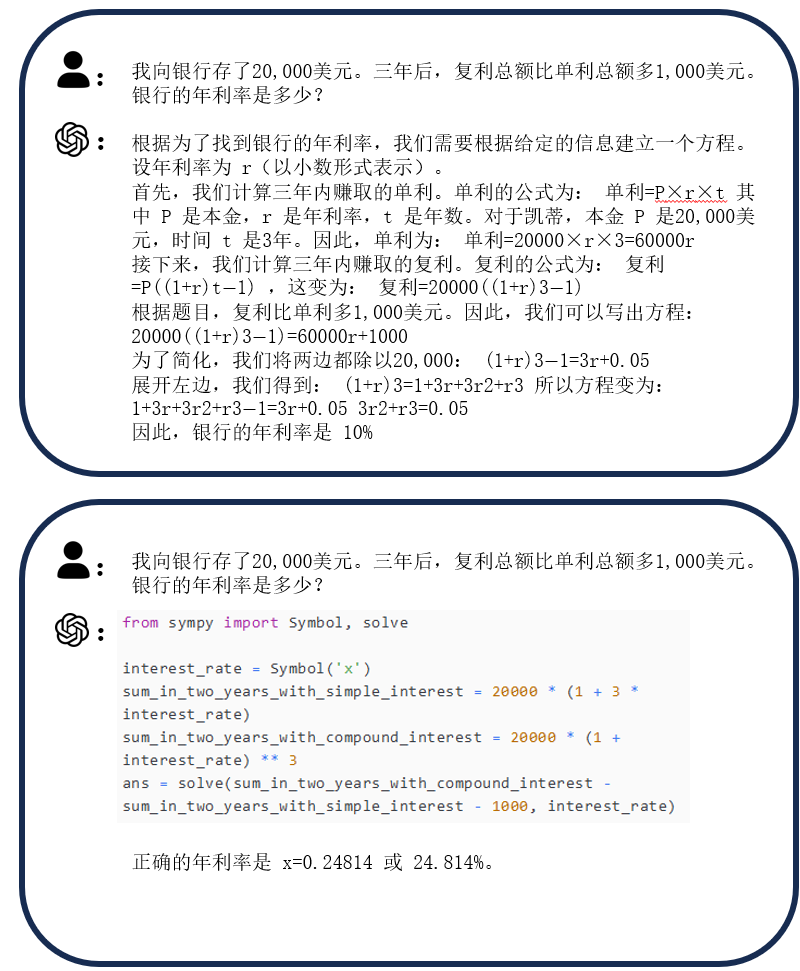
\includegraphics[width=0.7\textwidth]{大模型对数学问题的处理结果.png}
%     \bicaption{大模型对数学问题的处理结果}{Results of Mathematical Problem Processing by LLM}
%     \label{fig:4-1}
% \end{figure}
\begin{figure}[h]
    \centering
    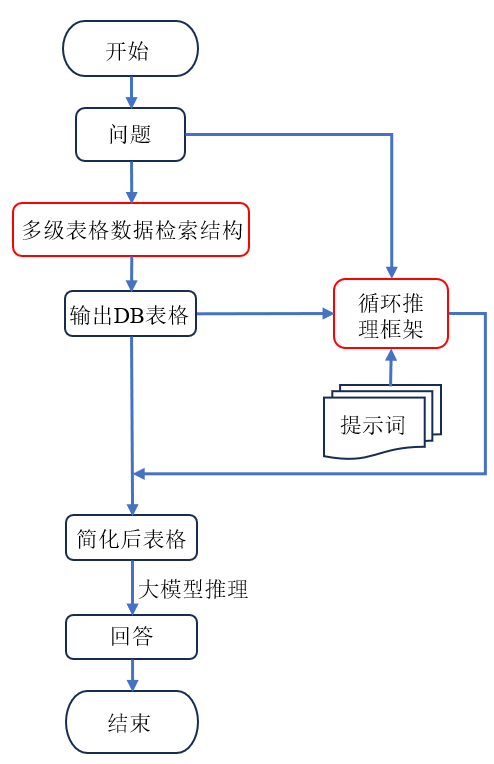
\includegraphics[width=0.54\textwidth]{整体框架.png}
    \bicaption{表格数据推理框架示意图}{Table Data Reasoning Framework}
    \label{fig:4-1}
\end{figure}

该框架针对RAG系统表格数据推理过程中的向量数据库构建环节和大模型推理环节进行了优化,如图\ref{fig:4-2}所示。提出了一种区别于传统单一向量数据库的包括多种文件格式在内的多级表格数据检索结构和针对表格文件SQL优化生成的循环推理框架,通过两个功能模块相互配合组成完整的表格推理框架。
\begin{figure}[h]
    \centering
    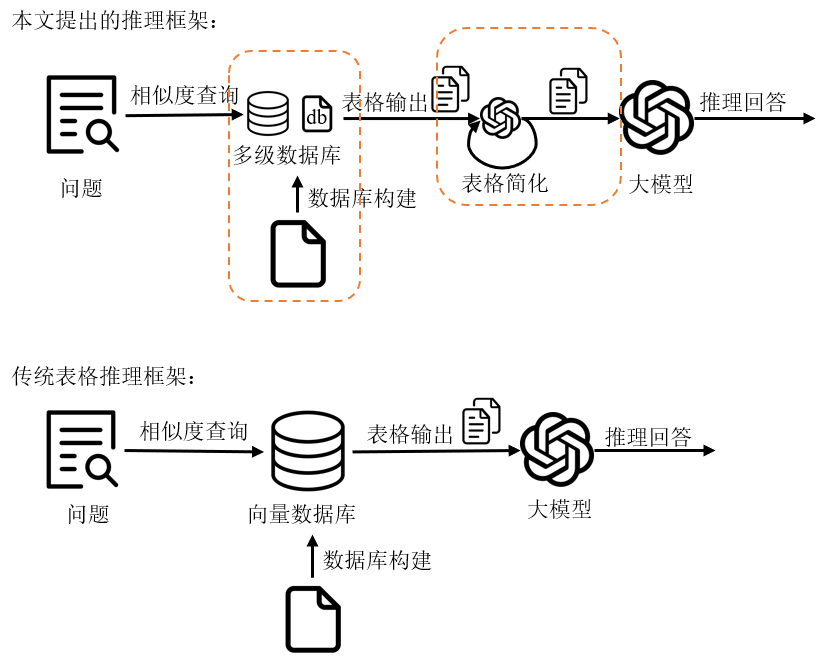
\includegraphics[width=0.74\textwidth]{推理框架对比.png}
    \bicaption{推理框架对比示意图}{Comparison of Reasoning Frameworks}
    \label{fig:4-2}
\end{figure}

% 同时,面对实际数据分析任务,表格数据输入模态多种多样包括excel表格、纯文本形式表格、数据库database表格和PDF表格等。针对多模态的表格文件主要存在两种处理方式,一种是将所有模态表格均以图片的形式输入大模型\cite{zheng2024multimodal},利用了LLaVA、Vit\cite{bang2023multitask,chen2023clip2scene,liu2023visual,radford2021learning,dosovitskiy2020image}等视觉编码模型将表格编码输入大模型,是一种端到端的方法,该方法即使在部分任务的表现上达到了最优,但是该方法缺乏可解释性、消耗计算资源过于庞大且依然不能解决大模型对数字信息的计算和推理能力;第二种方法是利用Agent代理的思想,利用外部接口来代替大模型处理数学问题并简化表格文件,提取关键信息。利用代理思想的方法拓展了大模型在解决问题时的功能多样性,将多种大模型不熟悉的如数字运算、数字推理等任务统一转化成代码生成任务,即大模型最擅长的任务。代理方法相对视觉编码的方法节约了大量训练算力,并且提高了大模型在任务中的可观测性和可解释性,是实际应用中的主流方法。
\subsection{表格数据预处理}
本小节介绍如何从未经处理的原始资料构建成框架中的多级表格检索结构。文件来源于隆德县水利局的水利调度业务资料,由于文件格式不统一,数据结构复杂,表格数据的行列关系复杂且存在多种模态的表格文件。为了保证后续框架的推理效率和准确性,需要对原始资料进行预处理,整体流程如图\ref{fig:4-3}所示。
第一步,对文本表格形式的资料进行OCR光学识别,提取表格数据,将所有表格数据转化成xls格式。由于OCR识别的准确率和效率受多种因素影响,如图片质量、文字清晰度、字体样式等,因此需要对OCR识别结果进行人工校验和修正,以确保数据的准确性和完整性。第二步,将xls文件按照表名-表头-数据的格式规范化、文本化,以便于后续处理。第三步,将处理后的表格数据通过python中的pandas表格处理工具转化为JSON格式,包括三个键值:表名、表头和数据。表名的键值类型为字符串,代表表格的名称;表头的键值为列表,列表中的每个元素为每列的列标题;数据的键值为二维列表,列表的每个元素为每行的数据信息构成的列表。第四步,通过python中的数据库函数接口,将JSON格式文件转化为database(DB)文件。最后,以每个表格为单位构建向量数据库,只将表名和表头向量化存储在向量数据库中,表格数据以文本形式、JSON和database的形式存储在本地。

\begin{figure}[h]
    \centering
    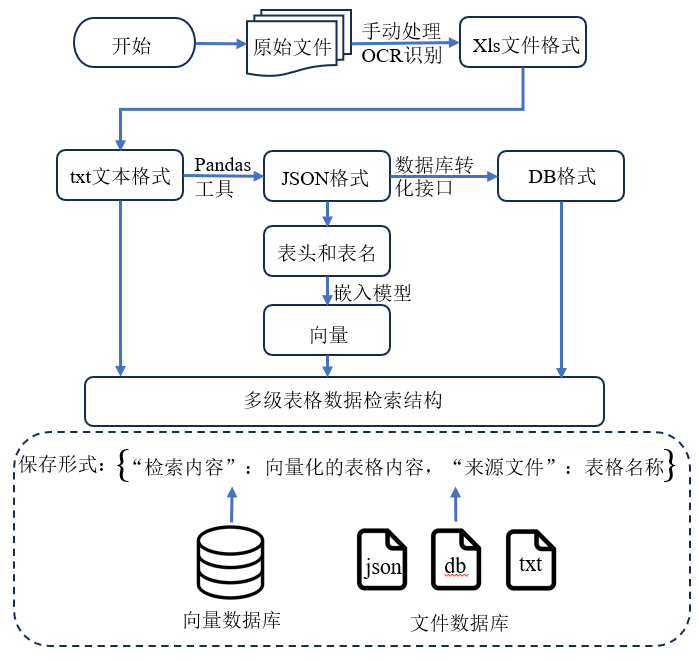
\includegraphics[width=0.82\textwidth]{表格处理流程.png}
    \bicaption{表格处理流程图}{Table Processing Flow Chart}
    \label{fig:4-3}
\end{figure}
\subsection{多级表格数据检索}

% 该方法主要包括对复杂表格数据的预处理、大模型的多轮推理以及外部SQL接口的使用。目前的主流表格推理框架默认所推理表格与问题的相关性,直接将具备回答问题所需信息的表格作为输入,测试框架的推理能力。但是在实际的推理任务中,需要通过文本向量相似性等方法对目标表格进行召回,为了提高召回精度同时保证大模型的推理的后续推理能够顺利进行,下面本章节提出一种多级表格数据目录检索方法。
上一小节中介绍了多级表格数据检索的结构以及构建方式,本小节介绍其创新点及其在RAG系统中的工作原理。

由于表格数据的数据结构特点,使用RAG系统中传统的文本预处理切块方式会导致返回的表格错误和表格不完整。传统文件处理的方式为,将表格数据以文本方式使用切块方法将表格以多个文本块的形式向量化存储在向量数据库中。由于表格文件的大部分信息均为数字,如果表格在中间截断,表格的中间部分以向量的形式存在,没有表头和表名,数据会丧失意义和信息。同样不同表格的中间数据部分会有相似的情况,若直接使用文本相似度检索非常容易将不同表格的数据信息混淆,削弱关键信息对于检索的影响从而区分不出表格来源之间的差别。表格数据之间相互区别的信息主要为表名和表头,这两个特征赋予数字实际意义,所以希望根据表头和表名信息构建数据向量库,同时也能够避免表格数据因长度过长被分割后,单独的数字信息丧失实际意义的问题。将过长的表格数据存储在向量数据库中也会在召回时浪费大量的相似度计算资源和延长响应时间。综上所述,本文设计了只将表名和表头向量化存储在向量数据库中,把表格的数据信息通过JSON和database的形式存储在本地,根据向量化检索后的文件来源进行本地表格定位,并且根据不同表的特征进行优化的表格召回方法。该方法可以提高表格召回的准确率和召回效率,并且可以保证将完整表格输入给大模型推理,同时为后续推理优化方法提供了格式化的表格文件,与传统处理方式的区别如表\ref{tab:方法对比}所示。
% \begin{figure}[!htbp]
%     \centering
%     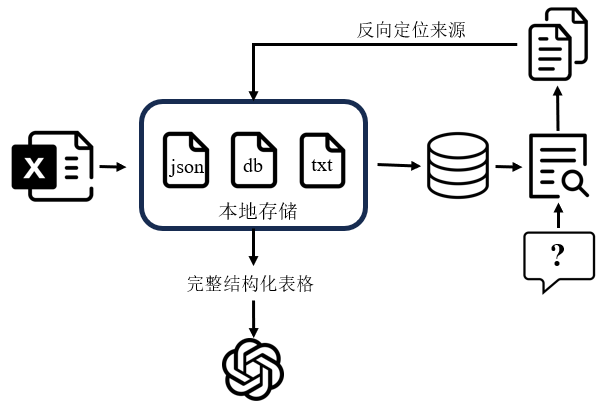
\includegraphics[width=0.66\textwidth]{表格检索框架示意图.png}
%     \bicaption{表格检索框架示意图}{Schematic Diagram of Table Retrieval Method}
%     \label{fig:4-2}
% \end{figure}
\begin{table}[h]
    \centering
    \bicaption{方法对比}{Method Comparison}
    \label{tab:方法对比}
    \begin{tabularx}{\linewidth}{@{}XXX@{}}
        \toprule[1.5pt]
        {处理方法} & {常规检索结构} & {多级检索结构} \\
        \midrule[1pt]
        分割单位 & 文本块 & 单个表格 \\
        嵌入内容 & 整个表格 & 表名和表头 \\
        存储形式 & 向量数据库 & 向量数据库及多种文件格式 \\
        返回类型 & 向量数据 & 向量数据和来源表格 \\
        \bottomrule[1.5pt]
    \end{tabularx}
\end{table}

该检索结构在RAG系统中的工作流程如图\ref{fig:4-4}所示。先通过向量相似度在向量数据库中返回对应表头表名向量,每一条对应的向量都包含一个特征来源文件(metadata),即这个向量数据是由哪个文件向量化而来。当输入的问题通过向量搜索模型匹配到目标表格时会直接定位到本地原始文件,根据需要提供JSON文件和database文件给后续框架进行推理等操作。
% 将表格文件转化为JSON、database和txt文本形式存储,再将txt文件中的表名和表头文本嵌入向量化,此时在向量数据库中,每一条对应的表头信息都包含一个特征来源文件(metadata),即这个向量数据是由哪个文件向量化而来。当输入的问题通过向量搜索模型匹配到目标表格时会直接定位到本地原始文件,根据需要提供JSON文件和database文件给后续框架进行推理等操作。
\begin{figure}[h]
    \centering
    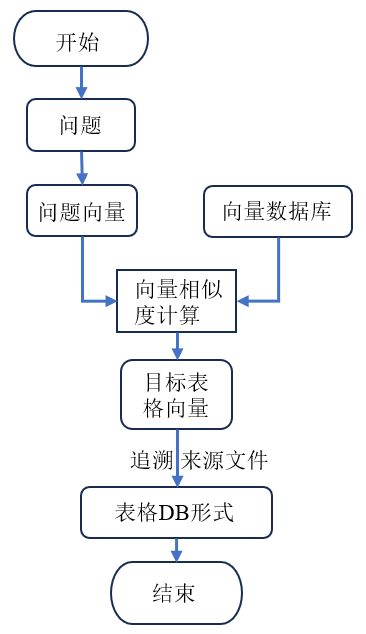
\includegraphics[width=0.42\textwidth]{表格检索过程流程图.png}
    \bicaption{表格检索过程流程图}{Table Retrieval Process Flow Chart}
    \label{fig:4-4}
\end{figure}
在向量检索中使用双塔检索结构\cite{bahdanau2015neural,sutskever2014sequence,fan2018hierarchical,holtzmancurious}。在召回过程中,双塔检索结构通过分阶段优化效率与精度,通常分为粗召回和精排序两个层级:粗召回阶段采用双塔神经网络架构,其中查询侧(Query Tower)和候选侧(Item Tower)分别通过独立编码器如Transformer,将问题文本编码为词向量,其中候选侧的编码过程为离线进行,在向量库构建时完成。再通过向量内积或余弦相似度计算初步匹配得分,并借助近似最近邻搜索(ANN)快速筛选Top-K候选集,实现计算效率与召回覆盖率的平衡;精排序阶段则引入复杂模型如第\ref{chap:第二章}章中介绍的BERT模型,对粗召回结果进行精细化相关性评估与排序,直接通过端到端的方式将问题和粗召回的候选向量输入,由模型输出相似度得分,从而在可控计算成本下提升整体召回质量。

\subsection{循环推理框架构建}
上一小结介绍了推理框架中的多级检索结构,检索根据问题能够返回正确的多种格式表格。本小节将介绍如何利用检索到的数据库DB表格等表格文件进行推理优化。
如上文提到,如果直接将上小节引入的检索方法检索到的表格输入给大模型会存在表格过长超出模型最大上下文长度和大模型对表格数据推理能力差的问题。可以通过引入Agent代理思想,通过SQL执行来处理表格,通过将数据精简减少表格长度和推理难度的方式提高回答质量,同时也使用SQL的计算能力来弥补大模型对数字关系推理的不足。

Agent代理的核心思想之一是将复杂任务分解为多个简单任务,从而降低每一次大模型调用时面对任务的难度,进而提升回答质量。是由多个大模型分工合作共同完成一次推理任务。综上所述,提出一种大模型循环表格推理框架,利用大模型强大的代码生成能力和自纠错能力生成准确有意义的SQL代码,再由外部接口执行代码并循环以上操作,得到最后精简的数据供大模型推理生成最终答案。

单次调用大模型生成SQL结果需要统一格式并且尽量降低模型的输出丰富度,可以通过调整模型输入参数和设计特殊提示词模板来实现,模型可以通过temperature参数控制输出的丰富程度,temperature越高,生成的文本更多样,反之,生成的文本更确定,因此对于生成SQL的大模型temperature设置为0.8,因为既需要固定同一个表格同一个需求输出SQL的一致性,也需要适当提高针对同一个表格不同需求的多样性。而针对固定大模型的输出格式上,框架希望可以直接将输出的文本作为下一阶段推理的输入,所以需要输出为可直接运行的SQL代码。上述需求通过提示词来解决。

提示词作为大模型调用的关键一环,可以不经过训练只使用文字输入的形式让大模型了解任务的需求,具体原理介绍已经在第\ref{chap:第二章}章写明。在SQL生成的提示词中,需要满足以下要点:

首先明确提出任务需求,该大模型的推理任务是什么。其次令模型理解输入的表格具体结构。因为检索到的目标表格也是以提示词的形式作为输入给大模型,这涉及到上面提到的表格篇幅过长问题,既需要令大模型明白表格的全貌,又需要减少表格长度。这里同样借助SQL的能力,利用SQL中表格初始化代码代替整张表格来使大模型理解表格结构,同时将大模型的知识注意力引入SQL中,再截取表头和少量表格信息组成提示词。在生成可直接运行的SQL代码的过程中,若采用冗长的文本描述方法,会存在以下问题:一方面受限于文字表达能力的局限性,难以精准且简洁地描述SQL代码的生成逻辑与结构;另一方面,模型在理解与转化这些文本描述时,存在一定概率出现语义对齐不准确的问题,导致生成的SQL代码无法准确实现预期功能。为解决这一问题使用Few-shot learning少样本学习方法,通过少数训练样本直接以提示词的形式来规范输出格式。设计满足以上需求的提示词如图\ref{fig:4-5}所示。
\begin{figure}[h]
    \centering
    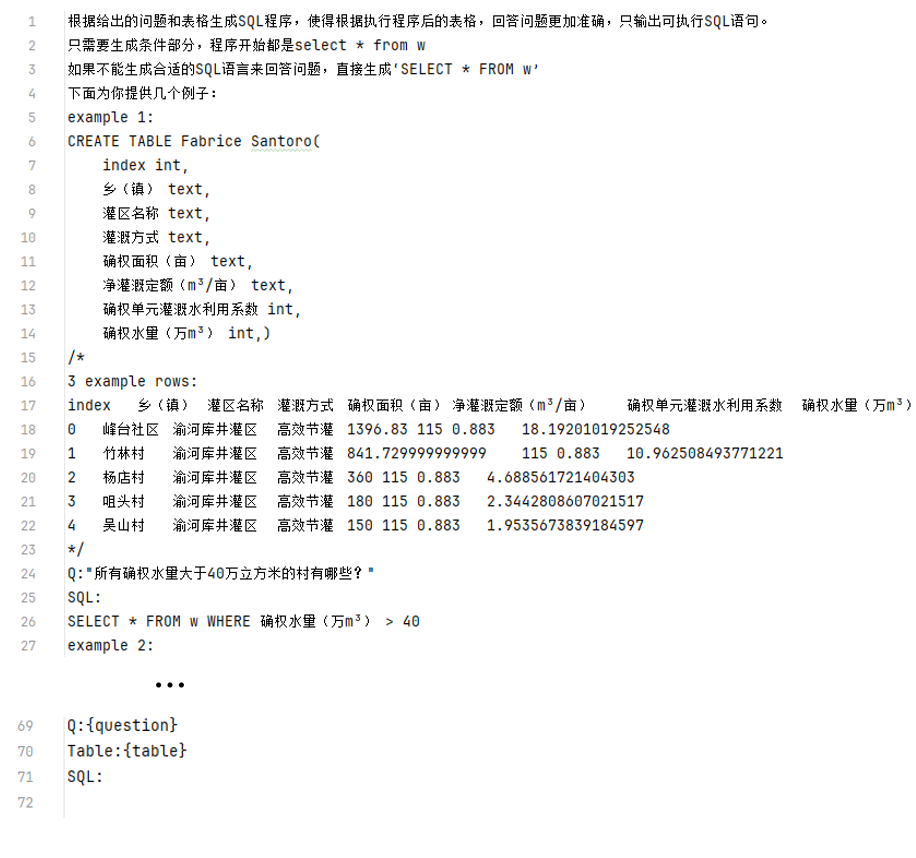
\includegraphics[width=0.85\textwidth]{SQL生成任务提示词.png}
    \bicaption{SQL生成任务提示词}{SQL Generation Task Prompt Words}
    \label{fig:4-5}
\end{figure}

提示词模板最后通过字典的格式将问题和文本化表格嵌入,由于少量输入输出例子,大模型会优先模仿并跟随前面的输出,就能保证输出SQL语句的一致性。如图\ref{fig:4-6}所示。
\begin{figure}[h]
    \centering
    \includegraphics[width=0.79\textwidth]{无few-shot.png}
    \bicaption{无少样本学习的SQL生成}{ SQL generation without Few-shot learning}
    \label{fig:4-6}
\end{figure}
特别注意的是,嵌入提示词模板的表格数据都将是以图\ref{fig:4-5}中一样文本的形式,包括最后生成回答的推理过程,database的文件形式只用于在框架内部利用SQL生成简化后的表格。然而还是有概率会出现输出SQL命令执行出错的问题。这里需要利用大模型的代码理解能力与自纠错能力,设计一种大模型的多循环自反馈框架。
% \begin{figure}[h]
%     \centering
%     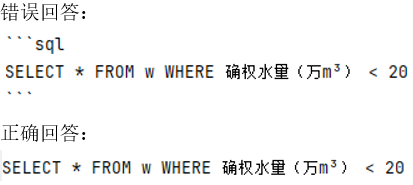
\includegraphics[width=0.5\textwidth]{SQL生成对比.png}
%     \bicaption{SQL生成对比}{Comparison of SQL Generation}
%     \label{fig:4-7}
% \end{figure}

该框架中设计的为三次循环反馈的自适应错误修正框架,其核心机制在于构建动态上下文感知的自纠正系统。将每次执行输出报错后的系统报错与前文组成上下文,生成包含完整错误的增强型上下文再输入模型。经过实际测试,将往次输入的报错和纠正共同组成上下文输入给模型非常关键,这样有助于令大模型意识到自身的错误方向和改进方向,若每次的报错信息单独输入给大模型会导致其原地踏步,孤立地处理离散错误事件。通过这种方法可以提高框架生成的SQL语法正确率。
% \begin{figure}[h]
%     \centering
%     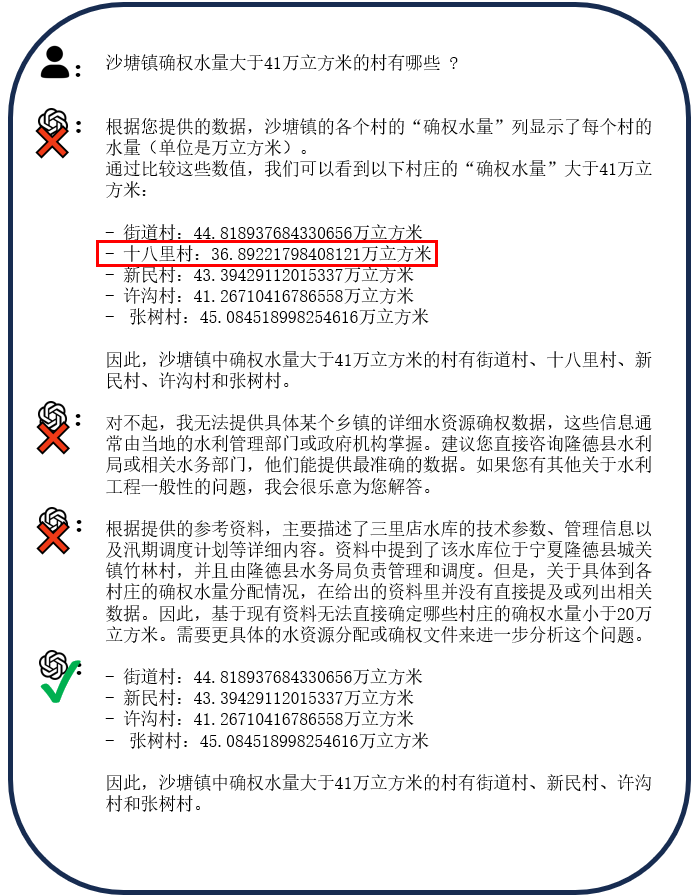
\includegraphics[width=0.8\textwidth]{回答对比.png}
%     \bicaption{优化前后回答对比}{ Comparison of Answers Before and After Optimization}
%     \label{fig:4-8}
% \end{figure}
当系统经历完整的三次迭代仍未能达成有效修正时,系统自动切换至为无优化的基础查询模式,直接执行select * from w全表扫描指令,将全部表格输出给下一步推理,来确保系统输出的完整性。这种双重模式切换机制在保证框架鲁棒性的同时,有效规避了因循环修正导致的潜在计算资源浪费问题。整体过程如图\ref{fig:4-8}所示。
\begin{figure}[h]
    \centering
    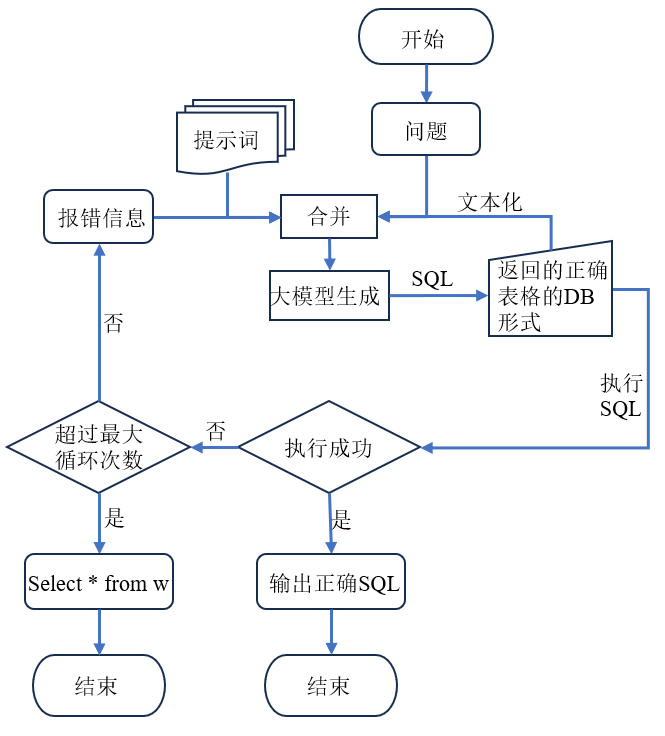
\includegraphics[width=0.66\textwidth]{循环推理流程图.png}
    \bicaption{循环推理框架流程图}{Flow Chart of Circular Reasoning Framework}
    \label{fig:4-8}
\end{figure}

\section{实验验证}
\subsection{数据集介绍及评价指标}
% 为验证章节提出的表格数据推理框架,本小结使用由隆德县水利局专家针对本地表格资料构建的问题集作为验证集,验证框架的优化效果。该问题集基于水利局本地资料,通过OCR光学识别和人工处理等方法将资料中存在的表格数据处理为xls格式,并根据专家经验设置问题,包括64个表格文件的110个水利业务中常见的,需要根据表格数据回答的问题。验证集中每条数据由问题、表格数据和表格名称组成,数据集未公开,具体样例见附录\ref{cha:问题集样例}。
为验证章节提出的表格数据推理框架,本小节设计两个实验分别验证多级表格检索结构对于目标表格检索的提升效果和循环推理框架对生成正确SQL的提升效果。

在多级表格推理的验证实验中,使用由隆德县水利局专家针对本地表格资料构建的问题集作为验证集。该问题集基于水利局本地资料,通过OCR光学识别和人工处理等方法将资料中存在的表格数据处理为xls格式,并根据专家经验设置问题,包括64个表格文件的110个水利业务中常见的,需要根据表格数据回答的问题。验证集中每条数据由问题、表格数据和表格名称组成,数据集未公开,具体样例见附录\ref{cha:问题集样例}。先通过检索构建方法将所有表格数据构建为向量数据库,测试输入为文本形式的问题,返回结果为表格数据来源也就是表格名称。通过对比检索得到的表格来源是否与验证集实际来源相同来衡量框架性能,相同为正例,不同为反例。准确度$P$的计算公式为
\begin{equation}
    P = \frac{C_{true}}{C_{total}} \times 100\%
\end{equation}
其中$C_{true}$为返回正确结果,$C_{total}$为总的检索结果。

循环推理框架的验证实验使用公开数据集WikiTQ\footnote[1]{\url{https://huggingface.co/datasets/afwull/WikiTQ}}。该数据集由WikiTableQuestions\cite{pasupat2015compositional}数据集衍生,表格从维基百科中选取,要求表格至少包含8行和5列。WikiTQ数据集由三部分组成:二维列表形式的表格数据、文本形式的针对表格的问题和回答。本实验中使用其中包含完整表格不缺失信息的3084条数据来验证框架对SQL生成语法正确性的的提升效果,将二维列表形式的表格文件通过多级检索框架转化成db形式,通过验证框架生成的SQL能否在db文件及数据库中正确执行来验证SQL的语法正确性。并且由于框架的功能特性,优化后不存在语法报错的SQL语句,而是作为错误SQL的代替,生成扫描全表的语句select * from w。实验通过对比优化前后能够正确执行的非扫描全表的SQL在所有SQL中的比例来验证框架的SQL生成能力。
% 先通过检索构建方法将所有表格数据构建为向量数据库,测试输入为文本形式的问题,返回结果为表格数据来源也就是表格名称。通过对比检索得到的表格来源是否与验证集实际来源相同来衡量框架性能。
% 根据该问题集设计两个实验分别验证表格检索和SQL生成的效果。表格检索实验中,先通过检索构建方法将所有表格数据构建为向量数据库,测试输入为文本形式的问题,返回结果为表格数据来源也就是表格名称。通过对比检索得到的表格来源是否与验证集实际来源相同来衡量框架性能,相同为正例(PE),不同为反例(NE)。SQL生成实验中,直接将表格和问题作为输入,返回结果为SQL语句。通过检查SQL语句是否符合语法、能否正确执行和是否能够优化表格数据来衡量框架性能。对于语法正确性指标,通过在数据库框架运行中是否报错为判断方法,顺利执行为正例,报错即为反例;对于SQL优化效果指标,由于SQL的生成无标准答案,无法直接进行对比,主要通过人为评估的方法将语法正确的SQL结果分为能优化和不能优化两类,能优化为正例,不能为反例。以上实验均使用准确度$P$为评价指标,计算公式为
% \begin{equation}
%     P = \frac{PE}{PE+NE} \times 100\%
% \end{equation}

实验中使用的嵌入模型为qwen-text-embedding-v2\footnote[2]{\url{https://github.com/QwenLM/Qwen}},精排序模型为bce-reranker-base\_v1\footnote[1]{\url{https://github.com/netease-youdao/BCEmbedding?tab=readme-ov-file}},大模型使用的是qwen-max和GPT-4-turbo\footnote[2]{\url{https://platform.openai.com/docs/models/gpt-4-turbo}}。数据库构建上使用FAISS作为向量数据库,分别对原始框架和优化框架进行试验对比效果。


% 本小结为证明推理框架对于SQL生成正确性的提升效果,也在公开数据集SQL\_Spider\_DDL\footnote[3]{\url{https://huggingface.co/datasets/philikai/SQL_Spider_DDL}}上进行了验证。该数据集在spider\cite{yu2018spider}数据集的基础上增加了数据库创建指令,提供了通过构造DB文件直接验证SQL正确性的能力。该数据集的验证集包括1.03k个由数据库构造代码、问题和问题对应SQL查询代码的数据组成。实验通过直接构造db文件并执行框架生成结果的方式验证生成SQL代码的语法正确性,统计执行正确的结果所占比例衡量框架性能。框架使用了qwen-max和GPT3.5-turbo两种模型测试框架效果。



\subsection{实验结果}
针对表格检索任务,对本章提出的多级表格检索方法和不进行特殊处理直接使用原始方法对比测试,
% 在测试中为了避免表格超出上下文长度导致的表格截断问题,只统计在大模型最大上下文长度内的表格与对应问题,
测试结果如表\ref{tab:table-retrival-results}所示。
根据实验结果显示,本章提出的多级表格检索方法在表格召回准确度上有明显提升,提高了对表格数据的检索能力。
% 同时也针对SQL的生成任务做出了测试,通过专家对测试结果的评估判断是否能够生成可执行、有优化效果的SQL。在实验中对于直接生成方式也进行了提示词辅助生成,测试结果如表\ref{tab:SQL-Generation-results}所示,其中SQL生成正确率代表框架生成的能够正确执行的SQL准确度,SQL生成恰当率代表框架生成的能够优化表格的SQL准确度。
\begin{table}[h]
    \centering
    \bicaption{表格检索实验结果}{Table Retrieval Experiment Results}
    \label{tab:table-retrival-results}
    \begin{tabularx}{\linewidth}{XXX}
        \toprule[1.5pt]
        {方法} & {原始方法} & {多级表格检索方法} \\
        \midrule[1pt]
        {准确度} & 66.3\% & 80.9\% \\
        \bottomrule[1.5pt]
    \end{tabularx}
\end{table}

在SQL生成实验中,对比原始方法和循环推理框架,使用Qwen-max和GPT-4-turbo两种大模型来验证。实验结果如表\ref{tab:sql-generation-comparison}所示,有效执行代表执行正确且不为select * from w的SQL占比,扫描全表为select * from w命令的占比。
% \begin{table}[h]
%     \centering
%     \bicaption{SQL生成实验结果}{SQL Generation Experiment Results}
%     \label{tab:SQL-Generation-results}
%     \begin{tabularx}{\linewidth}{XXX}
%         \toprule[1.5pt]
%         {方法} & {直接生成} & {循环推理框架} \\
%         \midrule[1pt]
%         {SQL生成正确率} & 46.3\% & 60.9\% \\
%         {SQL生成恰当率} & 30.9\% & 52.7\% \\
%         \bottomrule[1.5pt]
%     \end{tabularx}
% \end{table}
\begin{table}[htbp]
    \centering
    \bicaption{SQL生成实验结果对比}{SQL Generation Experiment Results Comparison}
    \label{tab:sql-generation-comparison}
    \setlength{\tabcolsep}{10pt} % 调整列间距
    \renewcommand{\arraystretch}{1.5} % 调整行间距
    \begin{tabularx}{\textwidth}{@{}cXXcX@{}}
        \toprule[1.5pt]
        \multirow{2}{*}{{模型}} & \multicolumn{2}{c}{{原始方法}} & \multicolumn{2}{c}{{循环推理框架}} \\
        \cmidrule(lr){2-3} \cmidrule(lr){4-5}
        & 有效执行 & 全表扫描 & 有效执行 & 全表扫描 \\
        \midrule[1pt]
        Qwen-max & 21.9\% & 63\% & 26.5\% & 73.5\% \\
        GPT-4-turbo & 27.1\% & 68.7\% & 29.3\% & 70.7\% \\
        \bottomrule[1.5pt]
    \end{tabularx}
\end{table}
实验结果表明,循环推理框架可以提高大模型对语法正确SQL的生成能力,并且不存在执行错误的情况,能够保证框架的完整性,避免了因SQL语法错误而导致的中断。
实验结果中优化前后生成全表扫面的SQL比例较高,原因主要有两点:1、数据集中表格数据本身无法获得正确信息来回答问题或表格已经为最简形式。2、无法生成正确SQL而达到循环推理次数达到最大值,直接生成扫描全表指令。原始方法中错误率也较低的原因是对于两种方法均包括了相同的提示词——“如果不能生成合适的SQL语言来回答问题,直接生成‘SELECT * FROM w’”,所以在相对困难的SQL生成任务中,会将部分错误SQL替换为全表扫描的SQL。

对于整体框架的具体框架推理回答效果的展示,通过一个信息查询任务回答展示具体效果,如图\ref{fig:4-9}所示。测试涉及对目标表格“隆德县农业灌溉用水确权汇总表”的召回和单特征数量关系的筛选。第一个回答为返回目标表格但无SQL优化回答,在回答中出现了错误答案,误将确权水量为36万立方米的十八里村输出;第二个回答由于在召回过程中,所有的向量相似度过低没有达到阈值,无表格返回;第三个回答为返回错误表格“三里店水库汛期调度运用计划表”导致;最后的回答为通过优化方法正确召回目标表格并使用推理框架得到正确数据的结果。由于最后输入给模型推理的表格只有符合要求的数据,所以避免了模型对数量关系不敏感的缺点,实现回答效果优化。
\begin{figure}[hb]
    \centering
    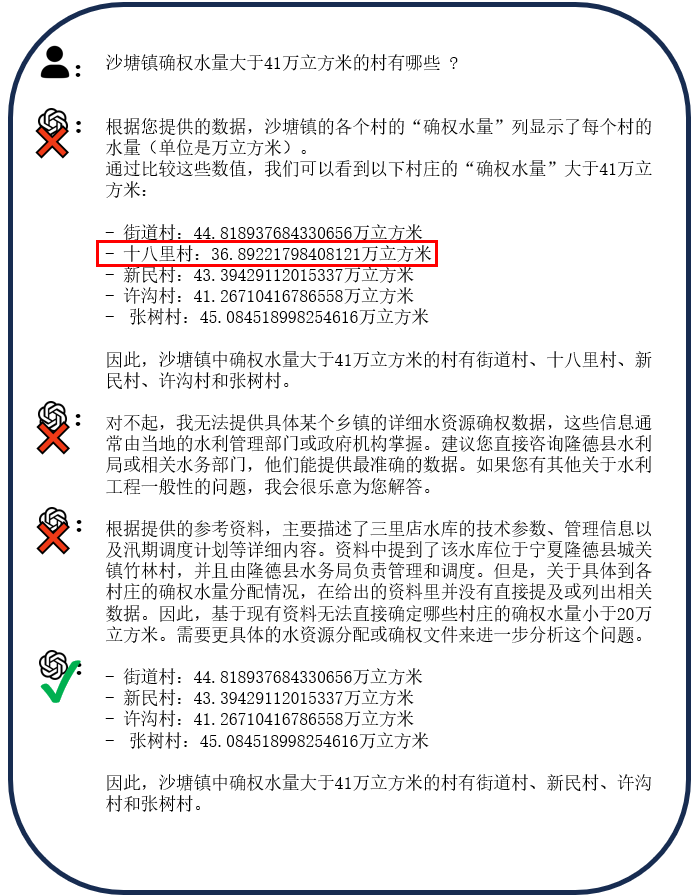
\includegraphics[width=0.58\textwidth]{回答对比.png}
    \bicaption{优化前后回答对比}{ Comparison of Answers Before and After Optimization}
    \label{fig:4-9}
\end{figure}
\section{本章小结}
本章节主要探讨了基于大模型的表格数据推理框架的设计,旨在提升大模型对结构化表格数据的理解与推理能力。通过深入分析表格数据的特点及大模型在处理表格数据时面临的挑战,提出了一种结合多级表格数据检索与循环推理的框架。

首先,针对表格数据的复杂性和大模型的局限性,设计了一种多级表格数据检索方法。该方法通过将表格的表名和表头信息向量化存储,避免了表格数据因长度过长而被分割的问题,提高了表格数据的召回准确率和效率。
其次,提出了一种大模型循环推理框架,通过引入Agent代理思想,将复杂任务分解为简单任务,降低了每次大模型调用时的推理难度。该框架利用大模型的代码生成能力,生成可执行的SQL代码,通过外部接口执行代码来简化表格数据,弥补了大模型在数字推理能力上的不足。此外,设计了一种多循环自反馈机制,通过动态上下文感知的自纠正系统,提高了推理的准确性。

通过上述方法,本章成功构建了一个表格数据推理框架,提升了大模型在处理结构化表格数据时的性能。这一框架不仅优化了表格数据的检索和推理过程,还为实际应用中的智能问答系统提供了强有力的技术支持。

本章所述内容已应用于学校合作企业的相关技术研发,并已提交专利申请。
